%%%%%%%%%%%%%%%%%%%%%%%%%%%%%%%%%%%%%%%%%%
%Copyright (C) 2018-2019 YuZJ.
%使用CC-BY-NC-SA授权。一份完整版本的许可证已位于附录。这个版本原始作者YuZJ,
%邮箱【邮箱】(最后连接于【时间】)。
%%%%%%%%%%%%%%%%%%%%%%%%%%%%%%%%%%%%%%%%%%
\documentclass{book}
\usepackage{xeCJK} %中文支持
\setCJKsansfont{SourceHanSansCN-ExtraLight.otf}
\setCJKmonofont{SourceCodePro-Light.otf}
\setCJKmainfont{SourceHanSerifSC-ExtraLight.otf}
\setCJKfamilyfont{bolded}{SourceHanSansSC-Bold.otf}
\renewcommand{\bf}{\CJKfamily{bolded}}  
\newcommand{\normalall}{\normalsize\normalfont\normalcolor}  
\usepackage{color}
\usepackage{graphicx}  %生成图片
\usepackage{geometry} %设置页面排版
\geometry{top=0.5in, bottom=0.5in, left=0.5in, right=0.5in, papersize={21cm,29.7cm}}
\usepackage[super]{nth} %生成序数词
\bibliographystyle{unsrt}
\usepackage{metalogo} %生成TeX标志
\usepackage{texnames} %生成TeX标志
\usepackage{fancybox} %生成带阴影的盒子
\shadowsize=2pt %配置盒子
\usepackage{shorttoc}
\usepackage{flafter}%使得所有浮动体不能被放置在其浮动环境之前
\usepackage{picinpar} %生成文本环绕
\usepackage{indentfirst}%生成段落
\usepackage[toc]{multitoc}%双栏目录
\usepackage{amssymb}%显示方块
\makeatletter\renewcommand{\verbatim@font}{\footnotesize \color{blue}\texttt} \makeatletter%修改verbatim环境格式
 %生成章节中文名和盒子
\renewcommand{\thechapter}{\arabic{chapter}}
\renewcommand{\thesection}{\arabic{chapter}.\arabic{section}}
\renewcommand{\thesubsection}{\arabic{chapter}.\arabic{section}.\arabic{subsection}}
\renewcommand{\thesubsubsection}{\arabic{chapter}.\arabic{section}.\arabic{subsection}.\arabic{subsubsection}}
\usepackage{titlesec}
\renewcommand{\bibname}{参考文献}
\renewcommand{\contentsname}{目录}
\renewcommand{\appendixname}{附录}
\titleformat{\chapter}[frame]{\bf \Huge}{\small 第 \thechapter 部分}{0pt}{}
\titleformat{\section}[frame]{\bf  \LARGE}{\small 第 \thesection 章}{0pt}{}
\titleformat{\subsection}[frame]{\bf  \Large}{\small  第\thesubsection 节}{0pt}{}
\titleformat{\subsubsection}[frame]{\bf \large}{\small 第\thesubsubsection 小节}{0pt}{}
\linespread{1.2} %行距命令
\usepackage{eso-pic}%背景图像命令
\usepackage[backref]{hyperref} %生成书签,这个应被放在末尾
\hypersetup{hidelinks,bookmarks=true,bookmarksopen=true,pdftitle=EMACS 26.2中文手册,pdfauthor=YuZJ}
\begin{document}
\setcounter{tocdepth}{5}
\begin{titlepage}	
\AddToShipoutPictureBG*{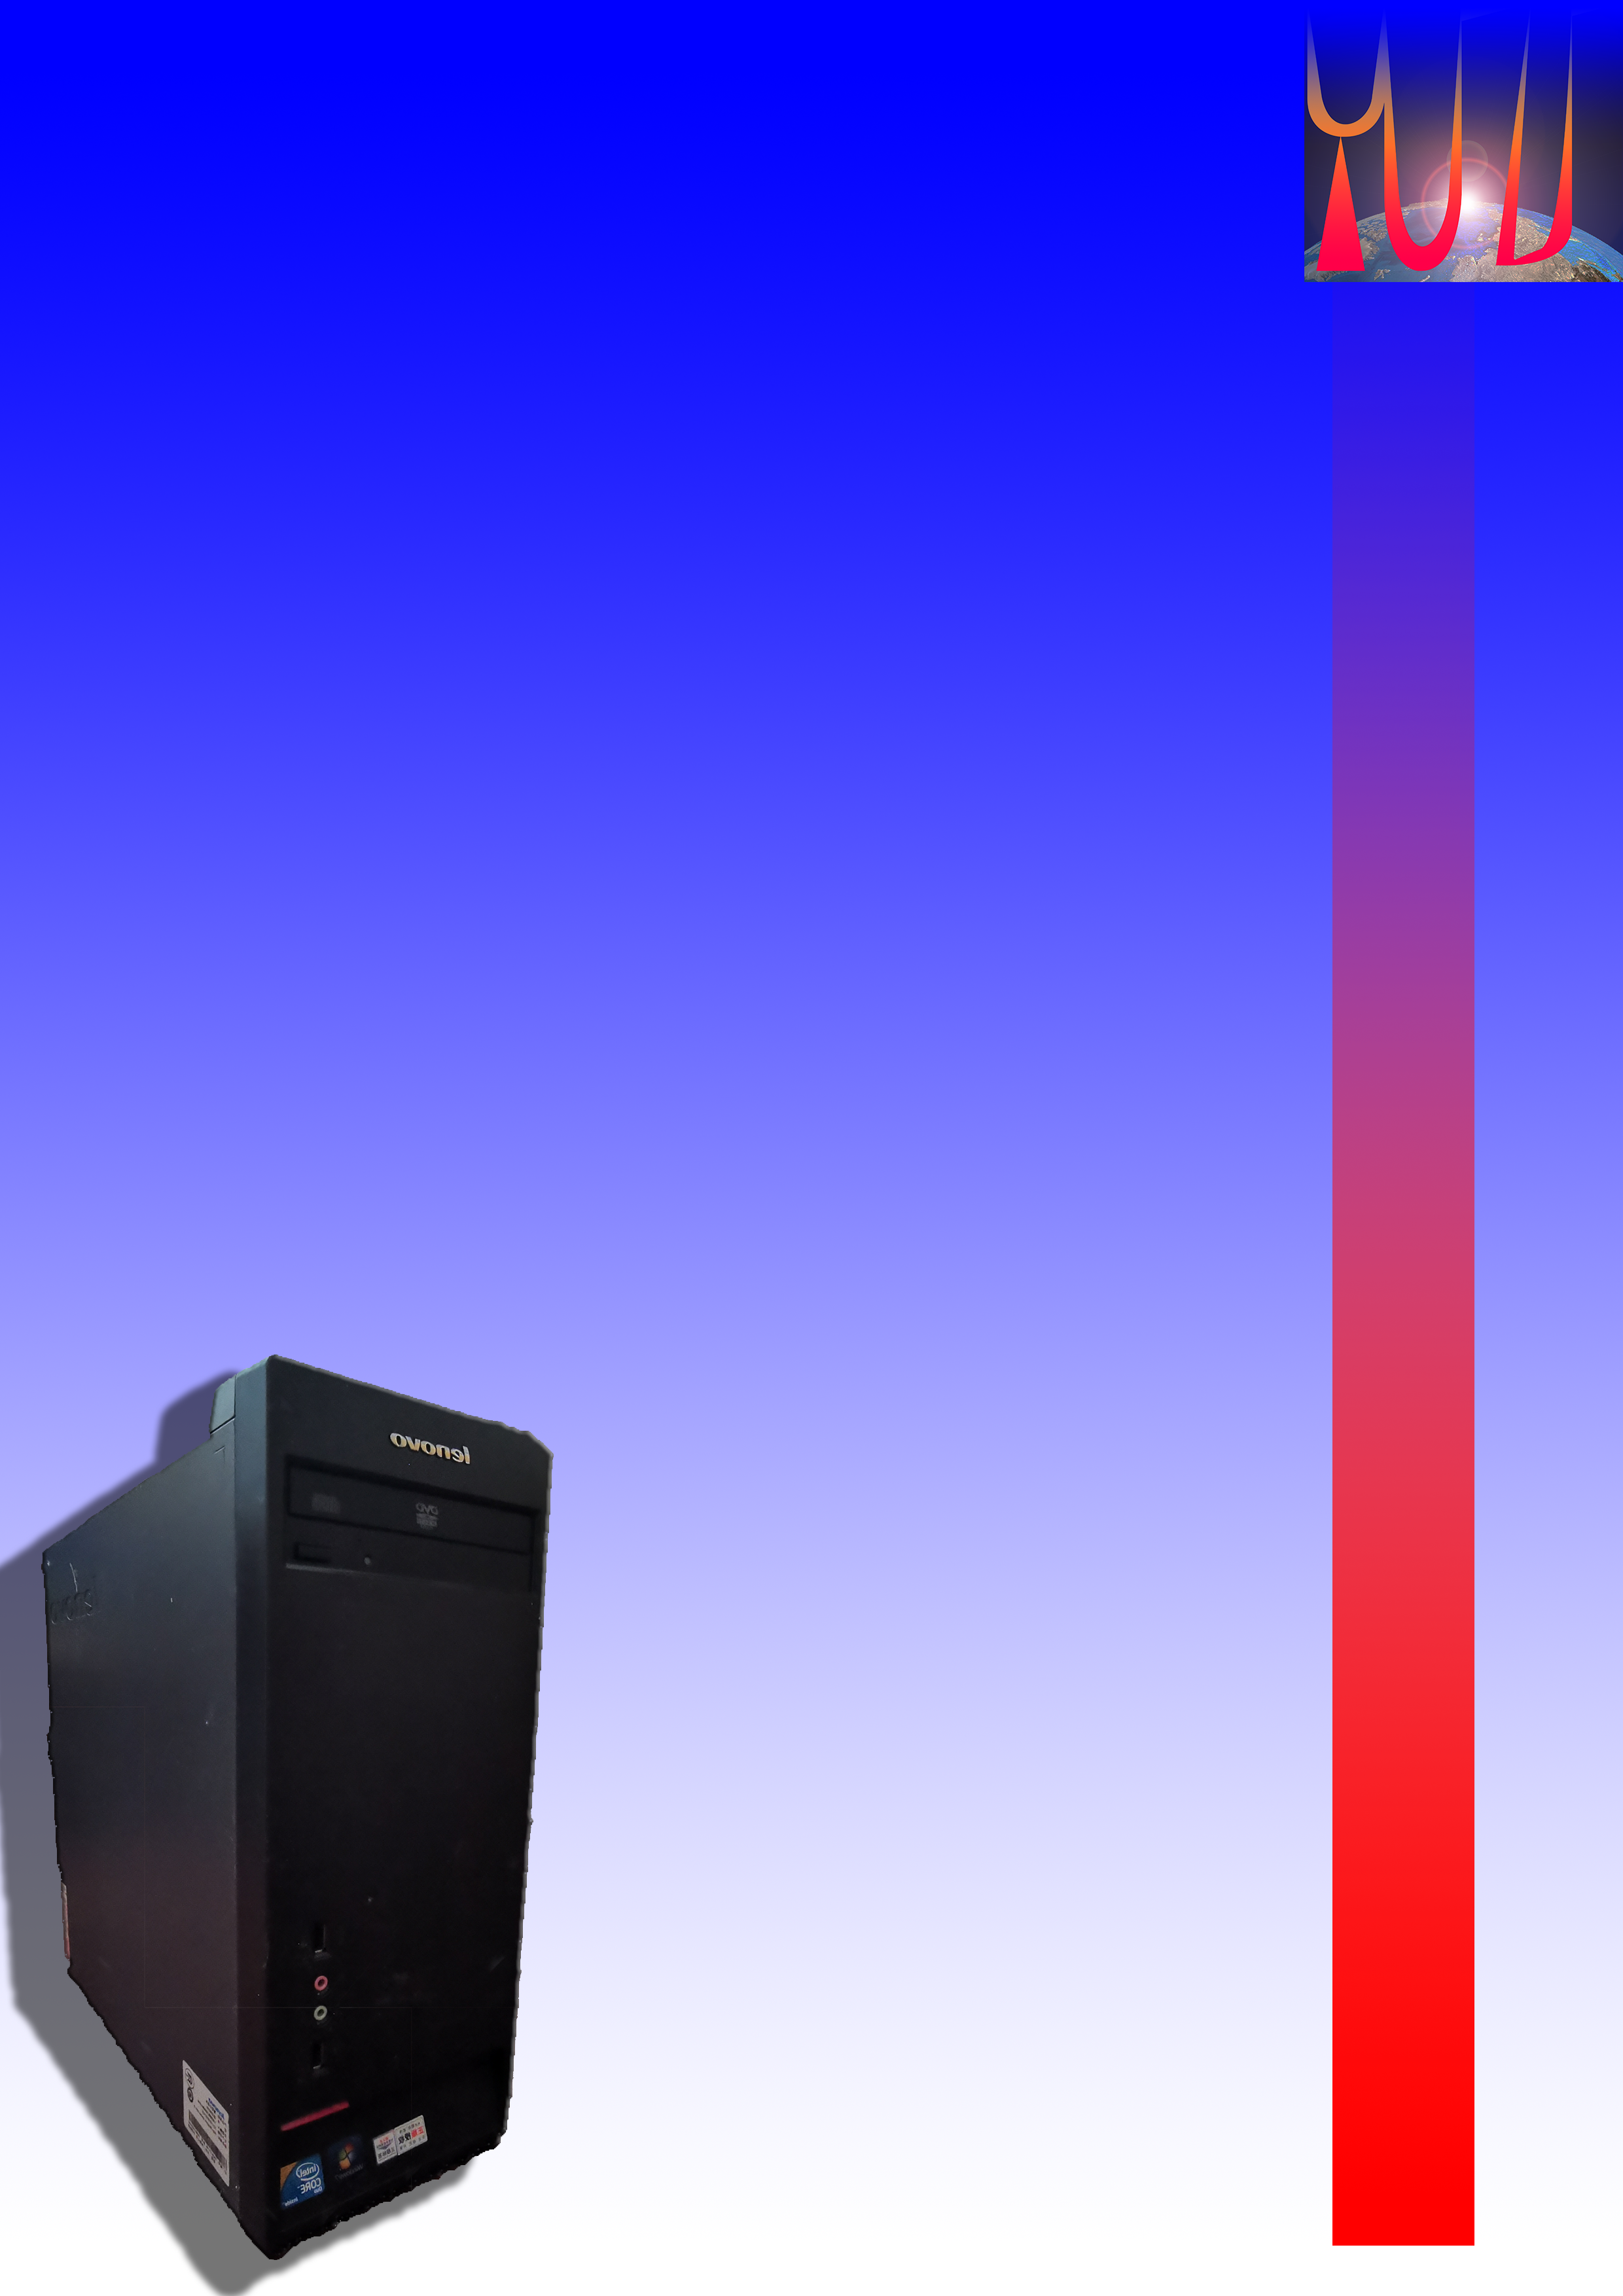
\includegraphics[width=21cm,height=29.7cm]{pic/face.png}}
{\color{white}{
\vspace*{10mm}
\begin{center}
\doublebox{\parbox{18cm}{
\begin{center}	
\Ovalbox{\Huge \bf EMACS 26.2中文手册\normalsize}\\\vspace*{5mm}\bf \large 作者:YuZJ \\\vspace*{5mm} 编译日期:\today	
\end{center}}}
\end{center}}}
\vspace*{25mm}\normalall
\shadowbox{\parbox[t]{8cm}{{\color{white}{【简介】}}}}
\end{titlepage}
\begin{center}
	\Huge \bf 【版本号】 \normalall
\end{center}
\shorttoc{简明目录}{1}
\tableofcontents
\chapter{The Organization of the Screen:屏幕的组织结构}
On a graphical display, such as on GNU/Linux using the X Window System, Emacs occupies
a graphical window. On a text terminal, Emacs occupies the entire terminal screen. We
will use the term frame to mean a graphical window or terminal screen occupied by Emacs.
Emacs behaves very similarly on both kinds of frames. It normally starts out with just one
frame, but you can create additional frames if you wish (see Chapter 18 [Frames]).
\par
在一个图形界面(例如,使用X Windows系统的GNU/Linux操作系统)中,Emacs占用了一个图形窗口(Window)。在一个文本终端中,Emacs占用了一整个终端屏幕。我们将会使用“窗体”(Frame)表示Emacs占用的图形窗体或终端屏幕。Emacs在这两种窗体下表现十分相似\footnote{译注:虽然我不这么认为}。一般情况下Emacs在启动时创建一个窗体,但是你可以按照你的意愿创建另外的窗体(参见第18章【窗体】)。\par
Each frame consists of several distinct regions. At the top of the frame is a menu bar,
which allows you to access commands via a series of menus. On a graphical display, directly
below the menu bar is a tool bar, a row of icons that perform editing commands when you
click on them. At the very bottom of the frame is an echo area, where informative messages
are displayed and where you enter information when Emacs asks for it.
\par
Emacs窗体包括多个区分明显的区域。在窗体的最顶端是菜单栏(Menu Bar),它允许你通过一系列菜单访问命令。在一个图形界面上,菜单栏下方是工具栏(Tool Bar)。它由一系列图标构成,当你单击它是它将执行编辑命令。回显区(Echo Area)窗体的最底端,用于显示Emacs的提示信息或者当Emacs需要你输入时键入信息。\par
The main area of the frame, below the tool bar (if one exists) and above the echo area, is
called the window. Henceforth in this manual, we will use the word “window” in this sense.
Graphical display systems commonly use the word “window” with a different meaning; but,
as stated above, we refer to those graphical windows as “frames”.
\par
在一个Emacs窗体中,位于工具栏(如果存在的话)以及回显区的大块区域称为窗格(Window)。此后我们将会使用“窗格”来表示这个意思。图形界面系统一般会使用“窗口”(Window)来表示不同的意思;但是,正如已经声明的一样,我们将称这些图形界面窗口为“窗体”(Frame)。\par
An Emacs window is where the buffer—the text or other graphics you are editing or
viewing—is displayed. On a graphical display, the window possesses a scroll bar on one
side, which can be used to scroll through the buffer. The last line of the window is a mode
line. This displays various information about what is going on in the buffer, such as whether
there are unsaved changes, the editing modes that are in use, the current line number, and
so forth.
\par
缓冲区(Buffer)——文本、图像以及其他你正在编辑或浏览的东西所显示的地方——位于Emacs窗口。在一个图形界面上,窗格\footnote{译注:是“Window”。此后窗格一律称“Window”,窗体一律称“Frame”。窗口?那是什么东西?}拥有一个纵向的滚动条用于滚动显示整个缓冲区。窗格的最底端一栏(在终端界面下是一行文字)称为状态栏(Mode Line),用于显示关于缓冲区中正在进行的操作的的信息,比如说是否有未保存的改变,正在使用的编辑模式(Editing Mode),当前的行号等等。\par
When you start Emacs, there is normally only one window in the frame. However, you
can subdivide this window horizontally or vertically to create multiple windows, each of
which can independently display a buffer (see Chapter 17 [Windows]).
\par
通常情况下,当你启动Emacs的时候,一个窗体中只有一个窗格。但是,你可以将这个窗格水平或竖直地分为多个窗格,它们各自独立地显示一个缓冲区(参见第17章【窗格】)。\par
At any time, one window is the selected window. On a graphical display, the selected
window shows a more prominent cursor (usually solid and blinking); other windows show a
less prominent cursor (usually a hollow box). On a text terminal, there is only one cursor,
which is shown in the selected window. The buffer displayed in the selected window is
called the current buffer, and it is where editing happens. Most Emacs commands implicitly
apply to the current buffer; the text displayed in unselected windows is mostly visible for
reference. If you use multiple frames on a graphical display, selecting a particular frame
selects a window in that frame.\par
在任何时候,有且仅有一个窗格是活动窗格(Selected Window)。在一个图形界面下,活动窗格显示一个更加明显的光标(Crusor)(一般是闪动的黑色方块“$\blacksquare$”);其它窗格显示一个不明显的光标(一般是空心方块“$\square$”)。终端界面只将在活动窗格显示一个光标。在活动窗格显示的缓冲区称为活动缓冲区(“Selected Buffer”)并且就是正在被编辑的缓冲区。大部分Emacs命令含蓄地作用于活动缓冲区;在非活动的缓冲区中显示的文字仅仅为参考而显示。如果你使用多窗体的图形界面,选择一个窗体再选择一个窗格。
\begin{center}
	\includegraphics[scale=0.4]{pic/Emacs-Terminal-Defaut}
\end{center}

\appendix
\renewcommand{\thechapter}{\arabic{chapter}}
\input{Appendix}
\addcontentsline{toc}{chapter}{参考文献}
\bibliography{Reference}
全书结束。
\end{document}
